% define macros
\def\d{\ensuremath{\,\mathrm{d}}}
\def\RP{\ensuremath{\mathcal{R}}}
\def\tR{\ensuremath{\widetilde{\mathcal{R}}}}
\def\far{\ensuremath{\mathcal{F}}}
\def\rsrc{\ensuremath{\widetilde{r}\,}}
\def\varH{\ensuremath{\mathrm{H}}}
\def\varL{\ensuremath{\mathrm{L}}}
\def\coincT{\ensuremath{\mathfrak{T}}}
\def\vT{\ensuremath{\mathcal{V}}}
\def\Tf{\ensuremath{\mathrm{T_f}}}
\def\th{\ensuremath{^{\mathrm{th}}}}


Once triggers have been obtained from the matched filter, re-weighted using the $\chi^2$ statistic, and vetted via coincidence test, they need to be evaluated for their statistical significance. In the low-mass CBC search we do this by computing a \ac{FAR} for each coincident trigger we obtain. This chapter details how that is done. We begin by reviewing properties of a Poisson distribution. Next, in section \ref{sec:coincidence_modelling}, we model the expected number of coincident triggers from single-\ac{IFO} distributions of a single template. In section \ref{sec:time_slide} we show how to using time-slides allows us to estimate the background to measure a \ac{FAR}. Section \ref{sec:multiple_templates} describes how we do this across the template space. In section \ref{sec:limitations} we discuss limitations in using time-slides to model the background.

\section{Poisson Process}
\label{sec:poisson}
If a system is a Poisson process, then on average, it will produce a mean number of events $\Lambda$ in a length of time $t$. The probability of getting $k$ events from this system in the same amount of time is:
\begin{equation}
\label{eqn:poison}
P(k|\Lambda) = \frac{\Lambda^k e^{-\Lambda}}{k!}
\end{equation}

$\Lambda$ is known as the \emph{rate parameter} of the system. It is a monotonically increasing function of time (for longer periods of time, we will expect a larger mean number of events). For a \emph{stationary} source $\Lambda$ will be linear in time. In other words, the mean number of events a stationary source would produce in several (hypothetical) iterations over the same period of time, $\tau$, will be the same as the mean number produced in several iterations over any other period of equal duration. For a \emph{non-stationary} source, the time dependence will be non-linear; i.e., two independent periods of time of equal duration would produce a different mean number of events. To get a duration-independent quantity, we define the source's \emph{rate density}, $\RP(t)$, which is the derivative of $\Lambda$ with respect to time:

\begin{equation}
\label{eqn:rate_param_def}
\mathcal{R}(t) \equiv \frac{\mathrm{d}\Lambda}{\mathrm{d}t}
\end{equation}

For stationary sources, $\RP(t)$ will be constant; for non-stationary sources, it will have a time dependence. The rate density is an \emph{intrinsic} parameter of the source: it depends on the source's physical characteristics and is independent of the duration of time it is observed for. (Contrast this with $\Lambda$, which mixes the intrinsic parameters with the period of time that the source is observed, which is an \emph{extrinsic} parameter). Whether or not a source produces a trigger in a given period of time is random; thus any measurement of the rate density is subject to uncertainty. We therefore define the ``true" rate density as the value obtained if an infinite number of independent measurements with identical initial conditions were carried out over the same duration of time:
\begin{equation}
\label{eqn:true_rate_param_def}
\widetilde{\mathcal{R}}(t) \equiv \lim_{N_m \to \infty} \frac{\sum_{k=1}^{N_m} \widehat{\mathcal{R}}(t)_{k}}{N_m}
\end{equation}
In this analysis we will denote ``true" rate densities by a tilde (e.g., $\tR$), measured values by a hat (e.g., $\widehat{\RP}$), and average values by a bar (e.g., $\overline{\RP}$).

If the source is stationary, then $\tR$ exists (at least theoretically; in practice, of course, we cannot perfrom an infinite number of measurements) and can be approximated by measuring $\RP$ in a series of experiments. If we observe a source for a period of time $t$, then, from \ref{eqn:rate_param_def}, the mean number of events produced during the experiment is:

\begin{eqnarray}
\Lambda & = & \int_{0}^{\Lambda}\, \mathrm{d}\Lambda' \nonumber \\
    & = & \int_{0}^{t} \tR(t')\, \mathrm{d}t' \\
    & \stackrel{=}{_{\tR(t') \rightarrow \tR}} & \tR t
\end{eqnarray}
$\widetilde{\RP} t$ is also the expectation value of the number of events:
\begin{eqnarray}
\mathbb{E}(N) & = & \sum_{k=1}^{\infty} k P(k|\Lambda) \nonumber \\
 & = & \sum_{k=1}^{\infty} k \frac{(\tR t)^k e^{-\tR t}}{k!} \nonumber \\
 & = & \tR t e^{-\tR t} \sum_{k=1}^{\infty} \frac{(\tR t)^{k-1}}{(k-1)!} \nonumber \\
 & = & \tR t e^{-\tR t} e^{\tR t} \nonumber \\
 & = & \tR t
\end{eqnarray}
Thus, in a single experiment, we can get a measurement of $\tR$ by simply dividing the number of events produced by the period. Averaging these measured values over $N_t$ experiments yields:

\begin{eqnarray}
\label{eqn:avg_rate_param}
\overline{\RP} & = & \frac{\sum_{k=1}^{N_t} t_k \widehat{\RP}_k}{\sum_{k=1}^{N_t} t_k} \nonumber \\
 & = & \frac{\sum_{k=1}^{N_t} t_k \left(\widehat{N}_k/t_k\right)}{\sum_{k=1}^{N_t} t_k} \nonumber \\
 & = & \frac{1}{\mathrm{T}}\sum_{k=1}^{N_t} N_k
 \end{eqnarray}
where $t_k$ and $\widehat{N}_k$ are the duration and number of triggers produced in the $k^{\mathrm{th}}$ experiment, and $\mathrm{T} = \sum_{k=1}^{N_t} t_k$. If the duration of each trial has roughly the same duration, $\tau$, then:

\begin{eqnarray}
\overline{\RP} & = & \frac{\sum_{k=1}^{\widehat{N}_t} N_k}{\tau N_t} \\
 & = & \frac{\overline{N}}{\tau}
 \end{eqnarray}
Since $\overline{N}$ is the mean number of events produced by a Poisson process, the variance is simply $\overline{N}$. Thus, the error in $\overline{\RP}$ is:
\begin{equation}
\label{eqn:err_R}
\delta \overline{\RP} = \frac{1}{\tau}\sqrt{\frac{\overline{N}}{N_t}}
\end{equation}

Once we have a measured value for $\RP$ we can estimate the probability of getting $k$ events from the source in any period $t$ (assuming the source is stationary); it is:

\begin{equation}
\label{eqn:prob_Rt}
P(k|\overline{\RP},t) = \frac{(\overline{\RP} t)^k e^{-\overline{\RP} t}}{k!}
\end{equation}
with error:

\begin{eqnarray}
\label{eqn:err_rate_param}
\delta P & = & \left| \frac{\d{P}}{\d{\overline{\RP}}} \right| \delta \overline{\RP} \nonumber \\
         & = & \frac{t}{\tau}\sqrt{\frac{\overline{N}}{N_t}} e^{-\overline{N}t/\tau} \left| \frac{\left(\overline{N}t/\tau \right)^{k-1}}{\left( k-1 \right)!} - \frac{\left(\overline{N}t/\tau \right)^{k}}{k!} \right|
\end{eqnarray}
In particular, we will be interested in the probability of getting one \emph{or more} events. This is:

\begin{eqnarray}
\label{eqn:one_or_more}
P(k\geq1 | \overline{\RP},t) & = & 1 - P(0 | \overline{\RP},t) \nonumber \\
 & = & 1 - e^{-\overline{\RP}t}
 \end{eqnarray}

If the source is non-stationary, then an exact value of $\tR(t)$ does not exist. This is due to the fact that it is impossible to distinguish between fluctuations in the number of triggers produced by a random process from statistical variation and flutuations due to a changing rate density. Since we can only do a finite number of experiments, in order to get a better measurement of $\RP$, we must observe it for a longer period of time. However, this results in a worse measurement of the time dependence of $\tR$, since any fluctuations that occur on a time scale smaller than the period of time we observe for will be indescernible. 

In this analysis, we will assume that the sources we observe are roughly stationary over the periods we observe them for. Although the interferometers do change over time, we leave it to other indicators, such as environmental and instrumental monitors, to inform us when these changes happen so that we can adjust our observation time accordingly.

\section{Modelling the Expected Number of Coincident Triggers}
\label{sec:coincidence_modelling}

Consider a coincident event produced by a network of detectors in an experiment with \emph{combined} \ac{SNR} $\rho^\dagger$. We wish to know the significance of the event; that is, we want to know the probability that the event was created by a specific source. To determine that probability we have two choices: we can compare the event to the distribution of the desired source's triggers or we can compare the event to a distribution of triggers from all other, \emph{background}, sources, which gives the \emph{false alarm probability}. Since we do not know \emph{a priori} the distribution of gravitational-wave triggers in the \acp{IFO}, in \ac{CBC} searches we aim to compute false alarm probabilities. We define the false alarm probibility, $P_F$, as being the probability of getting one or more triggers with a \ac{SNR} $\geq \rho^\dagger$ from a background distribution of triggers in the time searched, $\Tf$ (where ``$\mathrm{f}$" is used for \emph{foreground}). From equation \ref{eqn:one_or_more} this is:

\begin{equation}
P_F(k\geq1 | \far(\rho^\dagger), \Tf) = 1 - e^{-\far(\rho^\dagger) \Tf}
\end{equation}

$\far(\rho^\dagger)$ is the false alarm rate of a trigger with \ac{SNR} $\rho^\dagger$. It is the rate density of all background coincident triggers; i.e., it is the rate density of all coincident triggers occuring from every source except gravitational waves. Since we do not have an analytic model for the interferometers' noise sources we must measure $\far(\rho^\dagger)$ directly. To see how this is done, we first consider the true rate density of coincident triggers from \emph{all} sources in the \acp{IFO} (gravitational waves included), $\widetilde{\RP}_\mathrm{all}(\rho^\dagger)$. We then model the coincidence algorithm to derive this value. For simplicity, we only consider a single template; multiple templates are discussed in section \ref{sec:multiple_templates}.

Assuming stationary sources, in a single experiment of duration $\Tf$, $\widetilde{\RP}_\mathrm{all}(\rho^\dagger)$ is given by:
\begin{equation}
\label{eqn:rate_param}
\widetilde{\RP}_{\mathrm{all}}(\rho^\dagger) = \frac{\mathbb{E}\left(N_{\mathrm{uncorr}}(\rho^{\dagger2} \leq \sum_i\rho_i^2),\Tf\right) + \mathbb{E}\left(N_{\mathrm{corr}}(\rho^{\dagger2} \leq \sum_i\rho_i^2),\Tf\right)}{\Tf}
\end{equation}
Here, $\mathbb{E}\left(N_{\mathrm{uncorr}}(\rho^{\dagger2} \leq \sum_i\rho_i^2, \Tf)\right)$ is the expected number of triggers from all \emph{uncorrelated} sources that give a combined $\rho^2$ greater than or equal to $\rho^{\dagger2}$ in time $\Tf$. Uncorrelated means that a source that causes a trigger in one detector has no effect on the others. Conversely, $\mathbb{E}\left(N_{\mathrm{corr}}(\rho^{\dagger2} \leq \sum_i\rho_i^2, \Tf)\right)$ is the expected number of \emph{correlated} coincident triggers, which means they come from a source that causes triggers all of the detectors.

If we have $N_d$ detectors and $N_s$ independent trigger sources in each detector, then the expected number of \emph{uncorrelated} sources is given by:

\begin{eqnarray}
& & \mathbb{E}\left(N_{\mathrm{uncorr}}(\rho^{\dagger2} \leq \sum_i\rho_i^2, \Tf )\right) \nonumber \\
\label{eqn:N_general}
& = & \int\limits_{\substack{\rho^{\dagger2} \leq \sum_i\rho_i^2, \\ \rho_i \geq a ~ \forall i}}^{\infty}~~ \int\limits_{\substack{ |t_i - t_l| \leq \coincT_{i,l} \\ \forall l \neq i}}^{\Tf} \prod_i^{N_d} \sum_j^{N_s} \mathbb{E}\left(n_{i,j}(\rho_i,t_i) \right) \d t_i \d\rho_i \\ 
\label{eqn:N_general_prob}
& = & \int_{\mathcal{S}(\rho^\dagger)} \int_{\mathcal{T}(\Tf)} \prod_i^{N_d} \sum_j^{N_s}  \sum_{k=1}^{\infty} k\,P_{i,j}(k|\rho_i,t_i) \d t_i \d\rho_i 
\end{eqnarray}
$\mathbb{E}\left( n_{i,j}(\rho_i, t_i ) \right)$ in equation \ref{eqn:N_general} and $P_{i,j}(k|\rho_i,t_i)$ in equation \ref{eqn:N_general_prob} are, respectively, the expected number of triggers, and the probability of getting $k$ triggers, from the $j^{\mathrm{th}}$ source in the $i^{\mathrm{th}}$ detector with \ac{SNR} $\rho_i$ at time $t_i$. (In going from equation \ref{eqn:N_general} to equation \ref{eqn:N_general_prob} we have used the fact that the expected number of triggers produced by a source with \ac{PDF} $P(k)$ is $\sum_{k=1}^{\infty} k\,P(k)$.)

The regions of integration over $\rho$ and $t$ ($\mathcal{S}$ and $\mathcal{T}$, respectively) for a two-detector network are shown in Figure \ref{fig:snr_time_integrals}. The \ac{SNR} integral is carried out such that the quadruture sum of the single-\ac{IFO} \acp{SNR} are $\geq \rho^\dagger$, with a lower-cutoff at $a$. This lower cut-off is the \ac{SNR} cut that we impose in the matched-filter search; typically $a=5.5$. The time integral is carried out such that for each point in time in a given detector, $t_i$, we only integrate between $t_i \pm \coincT_{i,l}$ in every other detector. $\coincT_{i,l}$ is the duration of the coincidence window between the $i\th$ and the $l\th$ detector for the template we are considering. As dicussed in chapter \ref{ch:pipeline_principles} it is an \ac{SNR}-dependent quantity. However, since it is mostly dominated by the light-travel time between the $i\th$ and $l\th$ \ac{IFO}, here we approximate it to be a constant for each $(i,l)$ pair of detectors. 

$P_{i,j}(k|\rho_i,t_i)$ is a two-dimensional \ac{PDF}: it has some distribution in time and some distribution in $\rho$. If we assume the sources' time and $\rho$ dependence are independent of each other, then:

\begin{equation}
\label{eqn:twoDpdf}
P_{i,j}(k|\rho_i,t_i) = P(k|\rsrc_{i,j},t_i)P_{i,j}(\rho_i)
\end{equation}
In words: the probability of getting $k$ triggers from the $j\th$ source in the $i\th$ detector with \ac{SNR} $\rho_i$ in time $t_i$ is the probability of getting $k$ triggers from a source with rate-desnity $\rsrc_{i,j}$ in time $t_i$ times the probability of getting a trigger with \ac{SNR} $\rho_i$ from the source. If we again assume that all of the sources are stationary Poisson processes in the time domain, then:

\begin{equation}
\sum_{k=1}^{\infty} k P(k|\rsrc_{i,j},t_i) \d t_i = \rsrc_{i,j} \d t_i
\end{equation}
With this assumption, the time integral can be carried out independent of the integral over $\rho_i$; it gives the volume bounded by a hyper-surface, which we designate $\vT$:

\begin{equation}
\label{eqn:vTdef}
\vT(\Tf) \equiv \int\limits_{\substack{ |t_i - t_l| \leq \coincT_{i,l} \\ \forall l \neq i}}^{\Tf} \prod_i^{N_d} \d t_i
\end{equation}
$\vT$ has units of $[\mathrm{time}]^{N_d}$. Plugging this into equation \ref{eqn:N_general} we have:

\begin{equation}
\label{eqn:N_rate_general}
\mathbb{E}\left(N_{\mathrm{uncorr}}(\rho^{\dagger2} \leq \sum_i\rho_i^2, \Tf )\right) = \vT(\Tf) \int_{\sum_i\rho_i^2 \geq \rho^{\dagger2}} \prod_i^{N_d} \sum_j^{N_s} \rsrc_{i,j} P_{i,j}(\rho_i) \d\rho_i
\end{equation}

To estimate the expected number of coincident triggers with combined \ac{SNR} $\geq \rho^\dagger$ from \emph{correlated} sources, we assume that the sources create a trigger with the same $\rho$ at the same time (modulo the light-travel time) in all detectors. In this case, the expected number is the quadruture sum over the individual probabilities:

\begin{eqnarray}
\label{eqn:correlated_sources1}
\lefteqn{\mathbb{E}\left(N_{\mathrm{corr}} ( \rho^{\dagger2} \leq \sum_i\rho_i^2, \Tf ) \right) } \nonumber \\
 & = & \sum_{j=1}^{N_s} \sqrt{ \sum_{i=1}^{N_d} \left( \int_{\rho^{\dagger}/\sqrt{N_d}}^\infty \int_{0}^{\Tf} \mathbb{E}\left(n_{i,j}(\rho_i,t_i)\right)\d t_i \d \rho_i \right)^2 } \\
\label{eqn:correlated_sources2}
 & = & \Tf \sum_{j=1}^{N_s} \sqrt{ \sum_{i=1}^{N_d} \left( \rsrc_{i,j} \int_{\rho^\dagger/\sqrt{N_d}}^\infty P_{i,j}(\rho_i) \d \rho_i \right)^2 }
\end{eqnarray}
In going from \ref{eqn:correlated_sources1} to \ref{eqn:correlated_sources2} we have used equation \ref{eqn:twoDpdf} and have assumed the correlated sources are stationary. Since all triggers will occur in each detector within the light-travel time between them the constraints are removed from the time integral, making it simply $\Tf$. Likewise, as we have assumed that each source will create triggers with the same $\rho$ in all detectors, there are no constraints on the \ac{SNR} integral and the single-\ac{IFO} \ac{SNR} is reduced to $\rho^\dagger/\sqrt{N_d}$.

We assume that the only source that can create correlated triggers across detectors is from gravitational waves. Thus, the sum over the number of sources in equation \ref{eqn:correlated_sources2} becomes a single term, with $j = \mathrm{GW}$. This is a bit of an oversimplfication: due to the antenna patterns of the detectors and their varying sensitivies, a gravitational wave will only generate a trigger in all detectors with the same \ac{SNR} for certain sky locations and orientations. However, since we are interested in computing background rates in this analysis and not \ac{GW} rates, we will assume that the detectors are roughly co-located with similar sensitivity. Under this assumption, the $P_{i,\mathrm{GW}}$ is the same for all detectors; thus the integral can be pulled out of the sum, and we have:

\begin{equation}
\label{eqn:correlated_GW_colocated}
\mathbb{E}\left(N_{\mathrm{GW}} (\rho^{\dagger2} \leq  \sum_i\rho_i^2, \Tf ) \right) = \Tf \rsrc_{\mathrm{GW}}(\vec{\theta}) \sqrt{N_d} \int_{\rho^\dagger/\sqrt{N_d}}^{\infty} P_{\mathrm{GW}}(\rho) \d \rho
\end{equation}
Note that $\rsrc_{i,j}$ has been replaced by $\rsrc_{GW}(\vec{\theta})$. This is the rate of \acp{CBC} in the universe; as it depends on the parameters of the source, $\vec{\theta}$, we have made the parameter dependence explicit, even though we are still only considering a single template.

The integral in equation \ref{eqn:correlated_GW_colocated} gives the sensitivity of the detectors to \ac{GW} sources. To compute it, we need the dependence of the sensitivy as a function of $\rho$. This can be obtained as follows: we wish to know the number of sources the detector is sensitive to from here to some distance $D^\dagger$. If we assume that binary sources are distributed uniformly throughout space (which is a valid assumption for distances greater than $\sim10\,\mathrm{Mpc}$ and less than $\sim1\,\mathrm{Gpc}$ \cite{rates doc}), then this is:

\begin{equation}
(2.26)^{-3} \int_{0}^{D^\dagger} D^2 \d D \int \d\Omega
\end{equation}
where $\d\Omega$ is the solid angle. The factor $(2.26)^{-3}$ comes from approximating the volume enclosded by the detector's antenna pattern (which is peanut shaped) by a sphere with a radius equal to the detector's ``horizon distance". The ``horizon distance" is the distance to a binary with optimal orientation and location (i.e., it is the length of the longest part of the peanut) \cite{Finn and Chernoff}. As discussed in chapter \ref{ch:pipeline_principles}, the sensitive distance is related to \ac{SNR} by:

\begin{equation}
\label{eqn:DtoRho}
D = \frac{\sigma_{\mathrm{GW}}}{\rho}
\end{equation}
(The need for the ``$\mathrm{GW}$" subscript will become clear later.) Plugging this into the above, and setting $\rho^\dagger / \sqrt{N_d} = \sigma_{\mathrm{GW}} / D^\dagger$ we have:
\begin{equation}
(2.26)^{-3} \int_{0}^{D} D' \d D' \int d\Omega = \frac{4\pi}{(2.26)^3} \int_{\rho^\dagger/\sqrt{N_d}}^{\infty} \frac{\sigma_{\mathrm{GW}}^3 \d\rho}{\rho^4}
\end{equation}
Thus:
\begin{equation}
\label{eqn:GW_pdf}
P_{\mathrm{GW}}(\rho) = \frac{4\pi \sigma_{\mathrm{GW}}^3}{(2.26)^3} \rho^{-4}
\end{equation}
which gives:
\begin{equation}
\label{eqn:expectedN_GW}
\mathbb{E}\left(N_{\mathrm{GW}} (\rho^{\dagger2} \leq  \sum_i\rho_i^2, \Tf ) \right) = \frac{4}{3} \pi \frac{\sqrt{N_d}\, \sigma_{\mathrm{GW}}^3}{(2.26)^3 (\rho^\dagger/\sqrt{N_d})^3} \rsrc_{\mathrm{GW}}(\theta) \Tf 
\end{equation}
(Note that we only have one $\sigma_{\mathrm{GW}}^3$ in the equation. This is because we assumed that all the detectors had the same sensitivity. If we had not made this assumption, the $\sqrt{N_d}\,\sigma_{\mathrm{GW}}^3$ term would instead be $\sqrt{ \sum_i^{N_d} \sigma_{i,\mathrm{GW}}^6 }$.) Adding this term to equation \ref{eqn:N_rate_general} and dividing by $\Tf$ gives the overall rate-density $\widetilde{\RP}_{\mathrm{all}}(\rho^\dagger)$.

As an example, consider two arbitrary detectors, $\varH$ and $\varL$, that are roughly co-located and have similar sensitivies. Let us assume that each \ac{IFO} has only one non-gravitational wave source, which we call ``noise", and that this noise is Gaussian distributed in $\rho$ with some constant rate-density in time:
\begin{equation}
\mathbb{E}\left(n_{i,\mathrm{noise}}(\rho_i,t_i)\right)\d t_i \d\rho_i = \frac{\rsrc_{i,\mathrm{noise}}}{\sqrt{2\pi} \sigma_{i,\mathrm{noise}}} e^{-\rho_i^2 / 2\sigma_{i,\mathrm{noise}}^2} \d t_i \d\rho_i
\end{equation}
Given the large tail in the \ac{SNR} distribution, as seen in chapter \ref{ch:pipeline_principles}, it may seem absurd to make this assumption. However, if we use \emph{New \ac{SNR}} for our ranking statistic (which we still label $\rho$) instead of \emph{\ac{SNR}}, then, as seen in Figure \ref{fig:new_snr_dist} in Chapter \ref{ch:pipeline_principles}, this is not such a bad assumption, especially if the template we are considering is from a binary neutron star. The caveat is that the $\sigma_{i,\mathrm{noise}}$ in the above equation is not the same as the $\sigma_{\mathrm{GW}}$ in equations \ref{eqn:DtoRho}--\ref{eqn:expectedN_GW}. Although $\sigma_{\mathrm{GW}}$ is also the variance of the matched filter in Gaussian noise, that noise is for an \emph{idealized} detector that has a stationary Gaussian distribution in \ac{SNR}. The noise we are considering here comes from the actual detectors; as such, $\sigma_{i,\mathrm{noise}}$ can only be determined by fitting a Gaussian to the New \ac{SNR} distribution of the detector data. How, then, do we determine $\sigma_{\mathrm{GW}}$? Contrary to noise, we will assume that gravitational waves match the template well, resulting in $\chi^2 \approx 1$. In this case, New \ac{SNR} reduces to \ac{SNR}, and so we can use equation \ref{eqn:DtoRho} to relate $D$ to $\rho$. One other caveat is that we currently do not use a New \ac{SNR} cut as we do in \ac{SNR}. Due to the cut in \ac{SNR}, the distribution in Figure \ref{fig:new_snr_dist} ceases to be Gaussian and falls off at low New \ac{SNR}. For simplicity, we assume the same cut in New SNR here, and set $a = 5.5$.

With these assumptions in mind, the rate density of coincident triggers from all sources would be:

\begin{eqnarray}
\label{eqn:exampleSources}
\widetilde{\RP}_{\mathrm{all}}(\rho^\dagger) & = & \nonumber \\
&   & \frac{\coincT_{\varH\varL}(2\Tf - \coincT_{\varH\varL})}{\Tf} \frac{\rsrc_{\varH,\mathrm{noise}}\rsrc_{\varL,\mathrm{noise}}}{2\pi \sigma_{\varH,\mathrm{noise}} \sigma_{\varL,\mathrm{noise}}} \int_{\mathcal{S}} e^{-(\rho_{\varH}^2 / 2\sigma_{\varH,\mathrm{noise}}^2 + \rho_{\varL}^2 / 2\sigma_{\varL,\mathrm{noise}}^2 )} \d \rho_{\varH} \d \rho_{\varL} \nonumber \\
 & + & \frac{4}{3} \pi \frac{\sqrt{2} \sigma_{\mathrm{GW}}^2}{(2.26)^3 (\rho^\dagger / \sqrt{2})^3} \rsrc_{\mathrm{GW}}(\vec{\theta})
\end{eqnarray}

\begin{figure}[p]
\label{fig:snr_time_integral}
\begin{center}
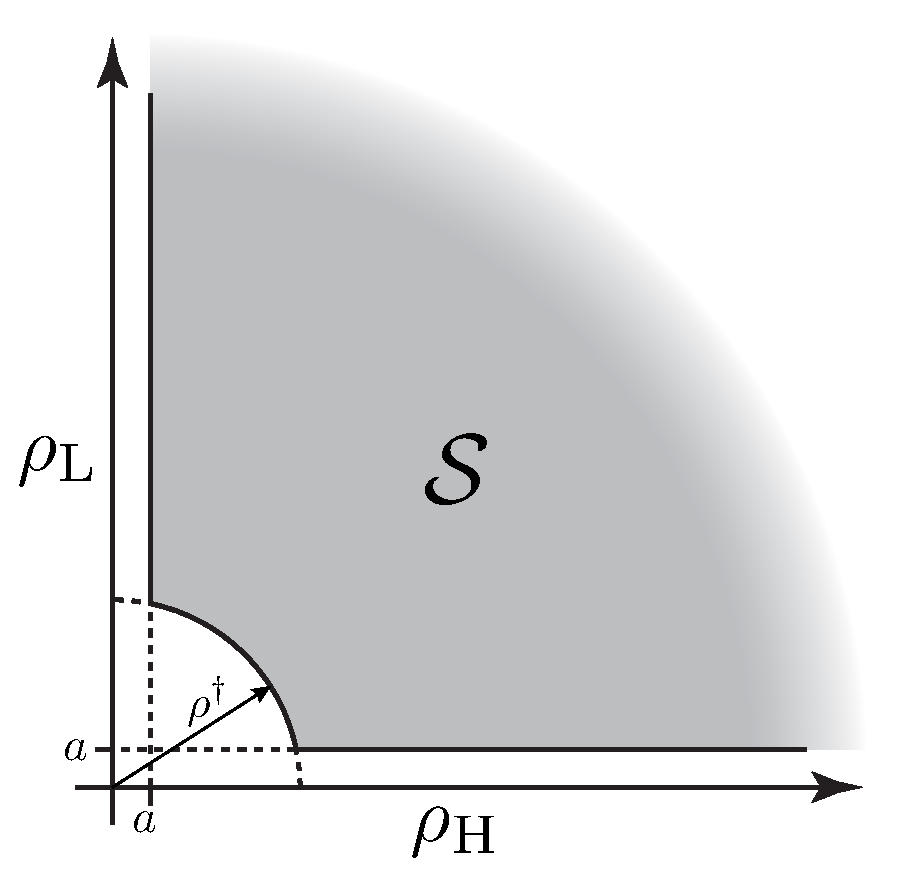
\includegraphics[height=4.25in]{figures/SNRintegrationRegion.pdf} \\
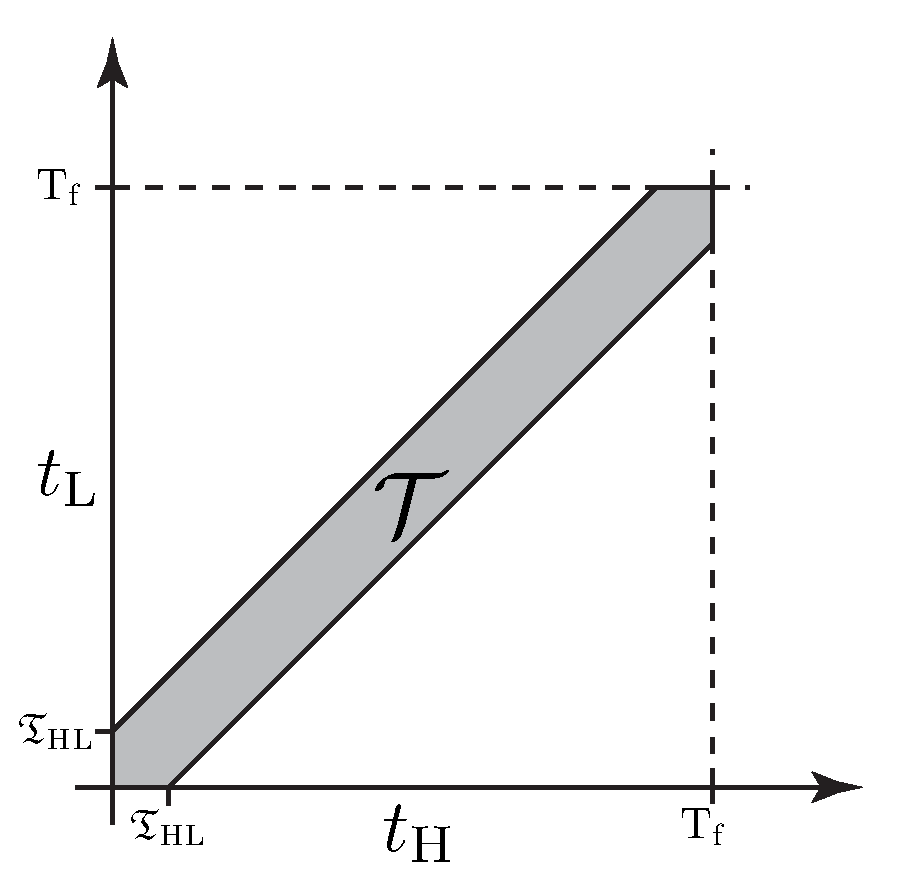
\includegraphics[height=4.25in]{figures/TimeIntegrationRegion.pdf}
\end{center}
\caption{The regions of integration in $\rho$, and time for a network of two detectors, $\varH$ and $\varL$.}
\end{figure}

\if{false}
For example, if we have two arbitrary detectors, $\varH$ and $\varL$, each with two independent sources $\gamma$ and $\delta$, then equation \ref{eqn:N_rate_general} would be:

\begin{eqnarray}
\label{eqn:exampleSources}
\lefteqn{ \mathbb{E}\left(N_{\mathrm{uncorr}}(\rho^{\dagger2} \leq \rho_\varH^2 + \rho_\varL^2, \Tf) \right) } \nonumber \\
 & = &  \vT(\mathrm{T_f}) \int_{\rho_\varH^2 + \rho_\varL^2 \geq \rho^{\dagger2}}  \d \rho_\varH \d \rho_\varL \times \nonumber \\
 & & \left(\rsrc_{\varH,\gamma}P_{\varH,\gamma}(\rho_\varH) + \rsrc_{\varH,\delta}P_{\varH,\delta}(\rho_\varH)\right) \left(\rsrc_{\varL,\gamma}P_{\varL,\gamma}(\rho_\varL) + \rsrc_{\varL,\delta}P_{\varL,\delta}(\rho_\varL)\right) \\ 
 & = & \coincT_{\varH\varL}(2\Tf - \coincT_{\varH\varL})\int_{\rho_\varH^2 + \rho_\varL^2 \geq \rho^{\dagger2}}  \d \rho_\varH \d \rho_\varL \times \nonumber \\
 & & \{ \rsrc_{\varH,\gamma}\rsrc_{\varL,\gamma}P_{\varH,\gamma}(\rho_\varH)P_{\varL,\gamma}(\rho_\varL) + \rsrc_{\varH,\gamma}\rsrc_{\varL,\delta}P_{\varH,\gamma}(\rho_\varH)P_{\varL,\delta}(\rho_\varL) + \nonumber \\
 & & \rsrc_{\varH,\delta}\rsrc_{\varL,\gamma}P_{\varH,\delta}(\rho_\varH)P_{\varL,\gamma}(\rho_\varL) + \rsrc_{\varH,\delta}\rsrc_{\varL,\delta}P_{\varH,\delta}(\rho_\varH)P_{\varL,\delta}(\rho_\varL) \}
\end{eqnarray}

\section{Computing Background Using Time Slides}

Since we wish to find the \ac{FAR}, $\widetilde{\far}$, and not $\widetilde{\RP}_{\mathrm{all}}$, the second (noise/GWs), third (GWs/noise), and fourth (GWs/GWs) terms above are a problem. Admiting gravitational wave sources into the background will give us a higher rate than the true rate $\widetilde{\far}$. The goal, then, is to remove \acp{GW} when computing the background rate.

This presents a problem: we do not know which triggers are due to gravitational waves and which are not (if we did, we would not have to do all this). Worse, the triggers that we are trying to compute false alarm rates for come from the same distribution of single \ac{IFO} triggers as the background rate that we use. To get around these difficulties, we can employ a few things we know about the physics of gravitational waves.

We know that a gravitational wave will arrive at all \ac{IFO}s within the light travel time between them. Therefore if we add some time offset, $\Delta t$ to each detector that is \emph{greater-than} the light-travel time between it and all other detectors but we only allow coincidences from triggers that are \emph{less-than} $\coincT$:
\begin{equation}
\label{eqn:time_constraint}
|t_i - (t_{i+1}+\Delta t)| \le \coincT_{i,i+1},~\Delta t > \coincT_{i,i+1}
\end{equation}
then we cannot get a coincidence from the same gravitational wave in all detectors. Adding the offset only allows gravitational waves that are coincident with \acp{GW} from other sources into the GWs/GWs term in equation \ref{eqn:mixed_source_terms}. While this can still present a problem, if our time searched is much less than the average rate of gravitational waves in the detectors, then the GWs/GWs term effectively goes to zero.

Adding a time offset has the additional advantage that we can repeat the experiment several times using the same data set to get an average value of $\far$, as long as the offet $\Delta t$ is large enough to ensure that each trial, or \emph{slide}, is independent of each other. The duration of each slide is the union of times that the \acp{IFO} are on after the offsets have been applied. If we do $N_{t}$ slides with each slide having duration $t_{k}$, then from equation \ref{eqn:avg_rate_param} we have:

\begin{equation}
\overline{\far} = \frac{\sum_{k=1}^{N_t} N_k\left(\rho^{\dagger2} \leq \sum_{i=1}^{N_d} \rho_i^2, \vec{\mathcal{O}}_k\right)}{\mathrm{T_{b}}}
\end{equation}
where $\mathrm{T_{b}} = \sum_{k=1}^{N_t}t_k$ is the total \emph{background} time. Here we have made the dependence on the time offset in each slide explicit by defining an \emph{offset-vector}:

\begin{equation}
\vec{\mathcal{O}}_k = \left[\Delta t_1 ~ \Delta t_2 ~ \ldots ~ \Delta t_{N_d} \right]_k %  \{\Delta t_i\}_k,~ i = 1, 2, \ldots, N_d
\end{equation}
which gives the time offsets of each detector in the $k^{\mathrm{th}}$ slide. If all the slides have the same duration, $\tau$, then, from equation \ref{eqn:err_R}, the error in the measurement of $\overline{\far}$ is:

\begin{equation}
\delta \overline{\far} = \frac{1}{\tau}\sqrt{\frac{\sum_{k=1}^{N_t} N_k}{N_t}}
\end{equation}

\section{Bias}
\label{sec:bias}

While the time-slide method gives a better estimate of $\far$, it introduces some bias. To quantify this, consider again equation \ref{eqn:N_general} for all sources. For simplicity, we intially consider only a single coincidence window. In this case, the time integral reduces to:

\begin{eqnarray}
\int_{|t_i - t_{i+1}| \le \coincT_{i,i+1}}^{\mathrm{T}=2\coincT_{i,i+1}}\prod_i^{N_d} \d t_i & = & \int_{-\coincT_{i,i+1}}^{\coincT_{i,i+1}} \prod_i^{N_d} \d t_i \nonumber \\
& = & 2 \prod_i^{N_d} \coincT_{i,i+1} \nonumber
\end{eqnarray}
since all points in time will be within the coincidence window. In the $p\th$ slide, equation \ref{eqn:N_general} becomes:

\begin{equation}
\mathbb{E}\left(N_{\mathrm{all}}(\rho^{\dagger2} \leq \sum_i\rho_i^2, 2\coincT )\right) = \int_{\sum_i\rho_i^2 \geq \rho^{\dagger2}} \prod_i^{N_d} \mathbb{E}\left(n_{i,\mathrm{all}}(\rho_i,t_i + \mathcal{O}_p[i] \pm \coincT_{i,i+1} ) \right) \d\rho_i
\end{equation}
To further simplify the problem, we consider the case in which $\rho^\dagger$


If we performed $N_t$ \emph{independent} experiments, then the expected number of triggers in this window would be:

\begin{equation}
\label{eqn:ideal_slides}
N_t \int_{\sum_i\rho_i^2 \geq \rho^{\dagger2}} \d \rho_i \prod_{i}^{N_d} \mathbb{E}( n_{i,\mathrm{all}}(\rho_i, t_i \pm \coincT_{i,i+1}) ) = N_t \int_{\sum_i\rho_i^2 \geq \rho^{\dagger2}} \d \rho_i \prod_{i}^{N_d} \sum_{k=1}^{\infty} k P(k|i,\mathrm{all}; \rho_i, t_i \pm \coincT_{i,i+1})
\end{equation}
When we perform time-slides, however, each of the slides are not truly independent. To see why, focus on one of the detectors, call it $\varH$, against which the other detectors are slid. In the first slide, the integrand is equation \ref{eqn:ideal_slides} (with $N_t = 1$). In each subsequent slide, the same expression will hold for all detectors aside from $\varH$, since, by sliding, we have introduced new data into the coincidence window. Yet because we are using the \emph{same} data in $\varH$, the probability of getting $k$ triggers in $\varH$ is \emph{not} $P(k|\varH,\mathrm{all}; \rho_i, \tau)$; instead, it is one if $k = n^{(0)}_{\varH}$ --- where $n^{(0)}_{\varH}$ is the number of triggers that occurred in $\varH$ in the first slide --- and zero otherwise. In other words, the \ac{PDF} in $\varH$ has collapsed around $n^{(0)}_\varH$. The expected number in the coincidence window is thus:

\begin{equation}
\label{eqn:actual_slides}
N_t \left(\prod_{i \neq \varH} \sum_{k=1}^{\infty} k P(k|i,\mathrm{all}; \rho_i, t_i \pm \coincT_{i,i+1})\right) \sum_{k=1}^{\infty} k \delta^{k}_{n^{(0)}_\varH} = N_t \prod_{i \neq \varH}^{N_d} \mathbb{E}( n_{i,\mathrm{all}}(\rho_i, t_i \pm \coincT_{i,i+1}) ) n^{(0)}_\varH
\end{equation}



%%%%%%%%%%%%%%%%%%%%%%%%%%%%
\if {false}
$m^{\mathrm{th}}$ noise source in the \varH~ detector and the $n^{\mathrm{th}}$ noise source in \varL. Let the true rate densities of these noise sources be $\widetilde{r}_{\varH,m}$ and $\widetilde{r}_{\varL,n}$, respectively. At a given time $t$, we will get a coincident trigger if there is at least one trigger from each source within $\coincT_{\varH\varL}$. The probability of getting atleast one coincident trigger is therefore:

\begin{eqnarray}
P(N_c \geq 1 | \widetilde{\rsrc}_{\varH,m}, \widetilde{\rsrc}_{\varL,n}, t \pm \coincT_{\varH\varL} ) &  & \nonumber \\
 & = & P(N \geq 1 | \widetilde{\rsrc}_{\varL,m},t \pm \coincT_{\varH\varL})P(N \geq 1 | \widetilde{\rsrc}_{\varL,m}, t \pm \coincT_{\varH\varL}) \nonumber \\
 & = & \left( 1 - e^{-\widetilde{\rsrc}_{\varH,m}2\coincT_{\varH\varL}} \right)\left( 1 - e^{-\widetilde{\rsrc}_{\varL,m}2\coincT_{\varH\varL}} \right)
\label{eqn:true_coinc_prob}
\end{eqnarray}
In equation \ref{eqn:true_coinc_prob} we have used the fact that the probability of getting one or more events from a Poisson distribution is:

\begin{eqnarray}
P(N \geq 1 | \RP, \tau) & = & 1 - P(0|\RP,\tau) \nonumber \\
    & = & 1 - e^{-\RP\tau}
\end{eqnarray}

Within a single slide, each block of coincident time can be considered to be an independent measure of the coincident $m,n$ rate density $\far_{m,n}$. Assuming $\far_{m,n}$ is constant across the duration of the slide, $\tau$, then we have $\tau/\coincT_{\varH\varL}$ measures of $\far_{m,n}$. However, this will not be sufficient to get a good approximation of $\widetilde{\far}_{m,n}$ especially if:

\begin{equation}
\widetilde{r}_{\varH,m}\widetilde{r}_{\varL,n} \left(\frac{\tau}{\coincT_{\varH\varL}}\right) < \frac{1}{\coincT_{\varH\varL}^2}
\end{equation}
In this case the expected number of events across the slide would be less than 1, making it likely that we would record no value and therfore end up with a mean value of zero for $\overline{\far}_{mn}$. For this reason, we extend the number of measures of $\far_{mn}$ we have by adding more slides.

However, the slides are not true indepedent measurements. Consider the same point in time in the $\varH$ detector as before, but now in the next slide. If this was a truly independent measurement, then the probability of getting one or more coincident triggers would again be equation \ref{eqn:true_coinc_prob}. The probability of getting a trigger during this period of time in $\varL$ would be the same it has been slid a period of time greater than $\coincT_{\varH\varL}$. The probability of getting a trigger in $\varH$, however, is \emph{not} the same. Since we are using the exact same period of time, it will be either 0 or 1, depending on whether or not we got a trigger in the first slide. Thus, the probability of getting a trigger at time $t$ for this and all subsequent slides is:

\begin{eqnarray}
P(N \geq 1|\widetilde{\rsrc}_{\varH,m}, \widetilde{\rsrc}_{\varL,n}, t \pm \coincT_{\varH\varL}, \mathcal{O}_{k \neq 1}) &  \nonumber \\
 = & \left\{
\begin{array}{l l}
1 - e^{-\widetilde{\rsrc}_{L,n}\coincT_{\varH\varL}} & \mbox{if $N_{\varH,m}(\mathcal{O}_1) \geq 1$} \\
0 & \mbox{if $N_{\varH,m}(\mathcal{O}_1) = 0$}
\end{array}
\right.
\end{eqnarray}

\fi
%In our ideal world of independent measurements, the probability that we will get atleast one coincident trigger with $\rho_c^2 \geq \rho^{\dagger2}$ at a time $t$ is given by the probability that we get one or more trigger in each detector within $\coincT$:

%\begin{equation}
%P(N \geq 1 | t, \{\widetilde{r}_{i,j}\}) = \prod_{i = 1}^{N_d} P(N \geq 1 | t\pm\Delta \coincT_{i}, \widetilde{r}_{i,n_i})
%\end{equation}

\fi

\end{document}
